\documentclass[../thesis.tex]{subfiles}

\begin{document}

\chapter{The Daya Bay experiment}
\label{chap:experim}

\section*{Introduction}

The Daya Bay experiment was designed to measure $\theta_{13}$ by observing the antineutrinos produced by the six 2.9~GW$_{\text{th}}$ nuclear reactors of the Daya Bay and Ling Ao power plants, located in Shenzhen in southern China. A total of eight functionally identical antineutrino detectors (ADs) were deployed, each containing a target of 20~tons of gadolinium-doped liquid scintillator (GdLS). Four of the ADs were evenly divided among two near halls ($\sim$350-600~m baselines from the cores), and the remaining four were placed in a single far hall ($\sim$1500-1950~m baselines). Shielding from cosmic rays was provided by $\sim$100~m and $\sim$300~m, respectively, of mountainous overburden at the near and far halls. The ADs in each hall were immersed in instrumented water pools which provided shielding from ambient radioactivity and detection of Cherenkov radiation from atmospheric muons. Redundant detection of muons, as well as directional information, were made available by resistive plate chambers (RPCs) laid on top of the water pools. In this chapter we discuss further details of the layout, the detectors, and the shielding and vetoing system of the experiment.

\section{Site layout}
\label{sec:expLayout}

\begin{figure}[ht]
  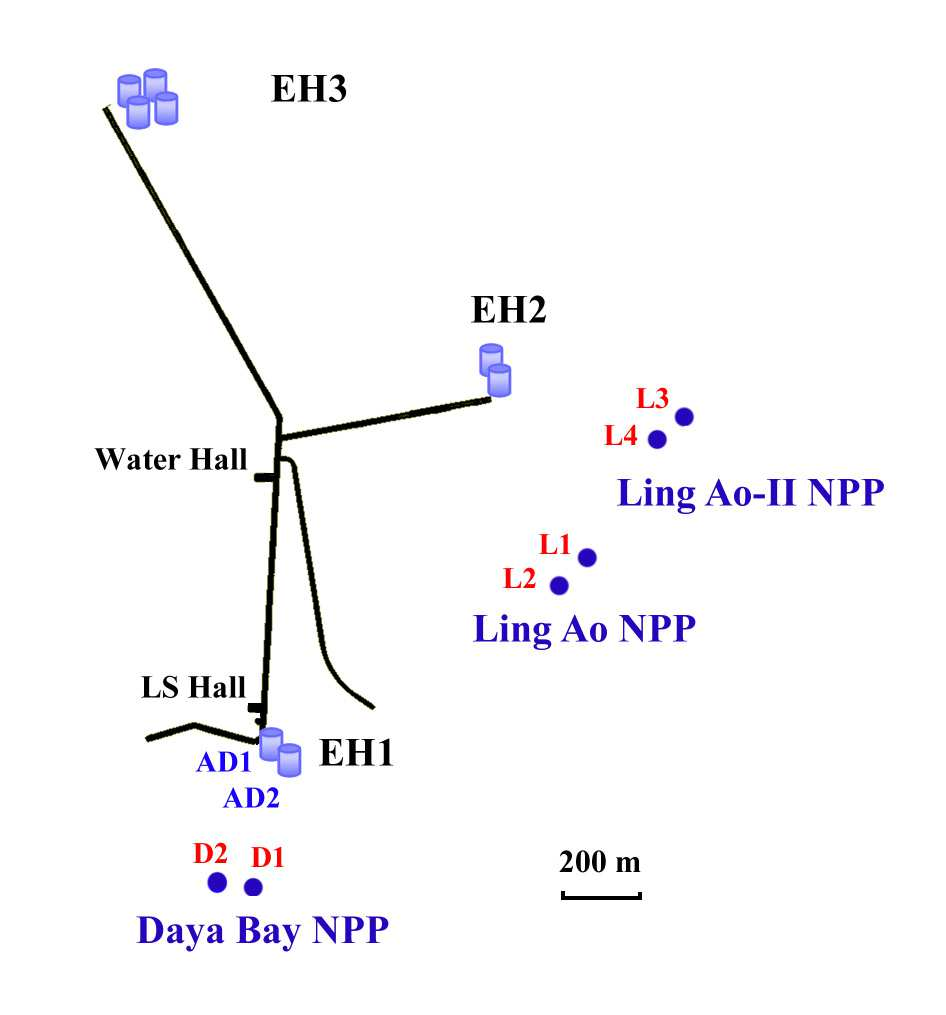
\includegraphics[width=0.5\textwidth]{layout.jpg}
  \caption{The layout of the Daya Bay experiment. The black lines represent horizontal tunnels into the mountain. From \cite{SideBySide}.}
  \label{fig:layout} 
\end{figure}

\begin{figure}[ht]
  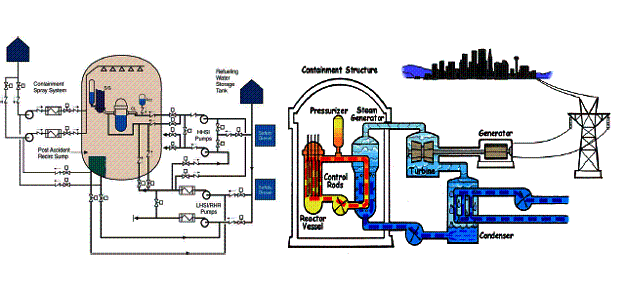
\includegraphics[scale=2.3]{cpr1000.png}
  \caption{The design of the CPR-1000 reactors used at the Ling Ao II power plant. The CPR-1000 is an upgraded variant of the similar M310 reactors used at the Daya Bay and Ling Ao I plants. From \cite{cpr1000}.}
  \label{fig:cpr1000} 
\end{figure}

As shown in \autoref{fig:layout}, the power reactors are divided into three nuclear power plants (NPPs), each containing two cores (illustrated in \autoref{fig:cpr1000}). One of the two clusters contains the Daya Bay NPP (cores D1 and D2), while the other cluster consists of the Ling Ao (L1 and L2) and Ling Ao-II (L3 and L4) NPPs. EH1 is located around 350~m from the Daya Bay NPP, while EH2 is roughly 500~m from the two Ling Ao NPPs. The far hall, EH3, in turn is located about 1900~m from the Daya Bay NPP and 1500~m from the Ling Ao NPPs. The measured baselines, as determined from a combined GPS and total station theodolite survey, are given in \autoref{tab:expBaselines}. The uncertainty of $\sim$2~cm in these measurements (less than 0.01\% in the worst case) is negligible relative to the other uncertainties in the oscillation analysis.  Likewise, simulations of reactor operation have determined that the centroid of $\nubar_e$ emission lies within $\sim$2~cm of each core's center \cite{An_2017}. Although $\nubar_e$ emission is distributed across the volume of each core (3.7~m high and 3~m in diameter), this spread has negligible effects at Daya Bay's baselines \cite{An_2017}\footnote{The same applies to the nonzero volume of the ADs}. Altogether, then, and in keeping with the official practices of the Collaboration, we treat each reactor as a point source, and we asume that the baselines are known exactly.

\begin{table}[ht]
  \begin{tabular}{lcrrrrrr}
    \toprule
    \multicolumn{2}{c}{} & \multicolumn{6}{c}{Reactor baseline [m]} \\
    \cmidrule{3-8}
    Hall & Detector & \multicolumn{1}{c}{D1} & \multicolumn{1}{c}{D2} & \multicolumn{1}{c}{L1} & \multicolumn{1}{c}{L2} & \multicolumn{1}{c}{L3} & \multicolumn{1}{c}{L4} \\
    \midrule
    EH1  & AD1      & 362.38  & 371.76  & 903.47  & 817.16  & 1353.62 & 1265.32 \\
         & AD2      & 357.94  & 368.41  & 903.35  & 816.90  & 1354.23 & 1265.89 \\
    EH2  & AD3      & 1332.48 & 1358.15 & 467.57  & 489.58  & 557.58  & 499.21  \\
         & AD8      & 1337.43 & 1362.88 & 472.97  & 495.35  & 558.71  & 501.07  \\
    EH3  & AD4      & 1919.63 & 1894.34 & 1533.18 & 1533.63 & 1551.38 & 1524.94 \\
         & AD5      & 1917.52 & 1891.98 & 1534.92 & 1535.03 & 1554.77 & 1528.05 \\
         & AD6      & 1925.26 & 1899.86 & 1538.93 & 1539.47 & 1556.34 & 1530.08 \\
         & AD7      & 1923.15 & 1897.51 & 1540.67 & 1540.87 & 1559.72 & 1533.18 \\
    \bottomrule
    % \multirow{2}{*}{EH1} & AD1      & 362.38  & 371.76  & 903.47  & 817.16  & 1353.62 & 1265.32 \\
  \end{tabular}
  \caption{Baselines between geometric centers of the ADs and of the reactor cores. From \cite{An_2017}.}
  \label{tab:expBaselines}
\end{table}

\section{Antineutrino detectors}
\label{sec:expADs}

\begin{figure}[ht]
  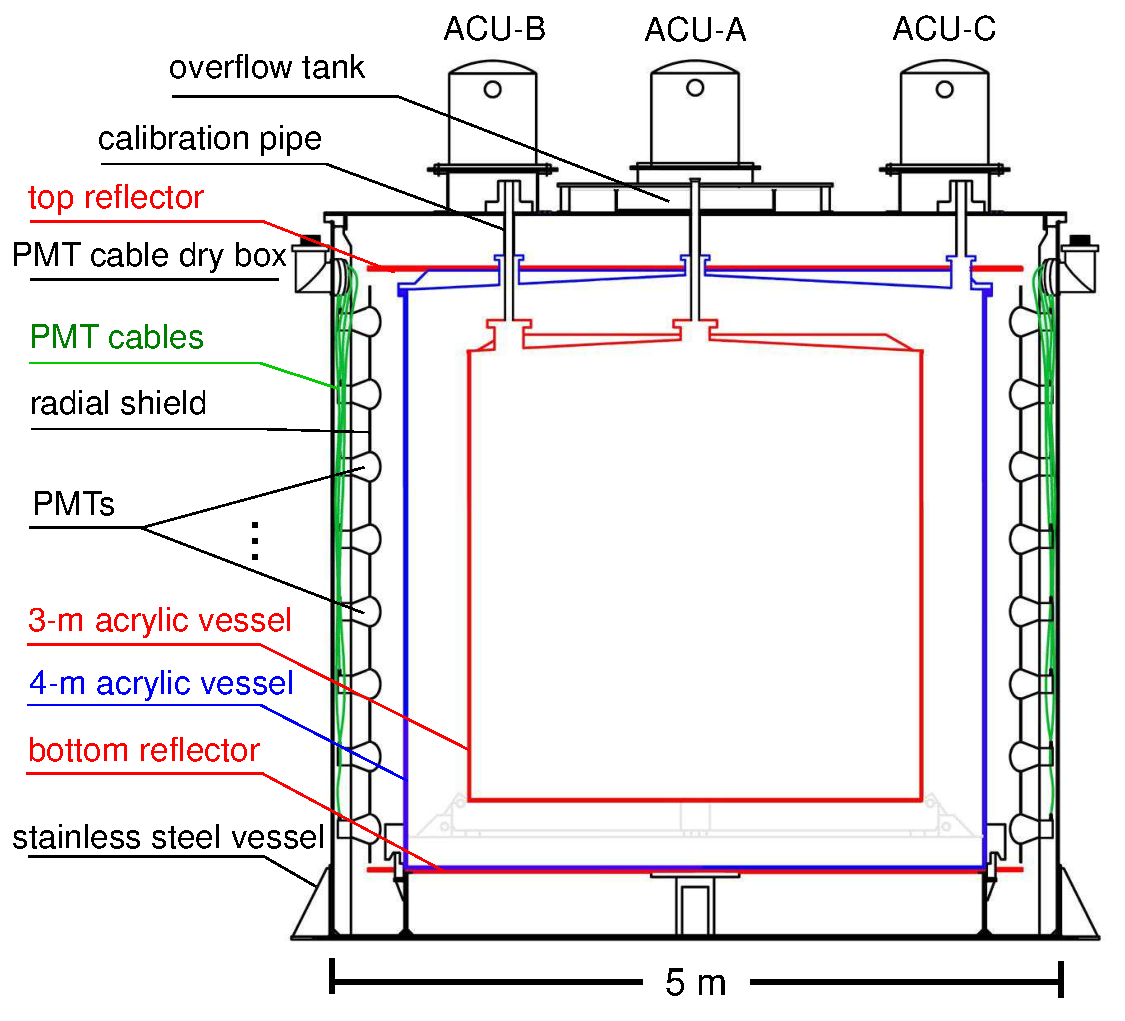
\includegraphics[scale=0.4]{exp_AD_structure.pdf}
  \caption{Structure of a Daya Bay antineutrino detector. From \cite{An_2017}.}
  \label{fig:expDetector}
\end{figure}

The design of the Daya Bay ADs is shown in \autoref{fig:expDetector}. Each AD is made of a cylindrical stainless steel vessel (SSV), 5~m in height and diameter, containing two nested cylinders of UV-transparent acrylic. The inner acrylic vessel (IAV), 3~m in height and diameter, 10~mm thick, contains the target mass of 20~t of gadolinium-doped liquid scintillator (GdLS)\footnote{Daya Bay's liquid scintillator consists of linear alkyl benzene (LAB) as the solvent, 3~g/L of 2,5-diphenyloxazole (PPO) as the fluor, and 15~mg/L of p-bis-(o-methylstyril)-benzene (bis-MSB) as the wavelength shifter. For the GdLS, $^{\text{nat}}$Gd was added in the form of a complex with 3,5,5-trimethylhexanoic acid (TMHA). Further details can be found in \cite{Beriguete_2014}.}, containing 0.1\% Gd by mass. Surrounding it is the outer acrylic vessel (OAV), 4~m in height and diameter, 18~mm thick, which contains 21~t of \emph{Gd-free} liquid scintillator (LS). This ``gamma catcher'' volume ensures the $\ge$90\% containment and measurement of gamma rays produced near the edge of the GdLS, while also providing additional target mass for studies that make use of neutron capture on hydrogen instead of on gadolinium. Between the OAV and the inner wall of the SSV, a 37~t volume of transparent mineral oil (MO) provides shielding from radioactivity in the detector materials, in addition to its role in balancing the stress on the OAV wall. All liquids were formulated to have densities within 1\% of each other (\autoref{tab:densities}), in order to minimize stresses on the vessel walls \cite{AN2016133}.

\begin{table}[ht]
  \begin{tabular}{lc}
    \toprule
    Liquid & Density (g/ml) \\
    \midrule
    Gd-LS & 0.860 \\
    LS & 0.859 \\
    MO & 0.851 \\
    \bottomrule
  \end{tabular}
  \caption{Densities of the liquids in the ADs \cite{SideBySide}.}
  \label{tab:densities}
\end{table}

Although the ADs were filled at different times (especially in the cases of EH2-AD2 and EH3-AD4, which were commissioned after the experiment had already begun taking data), each liquid (GdLS, LS, and MO) was prepared as one large batch in 2011 and kept in storage tanks that were subsequently used, in equal proportions, for all 8 ADs. This procedure minimized any variations in liquid properties between the ADs. Given that the antineutrino detection efficiency is directly proportional to the number of target protons (i.e., the mass) in the GdLS volume, it was crucial to accurately measure the liquid mass in each AD, as any errors in this step would translate into a bias on $\theta_{13}$. Toward this end, the filling process employed precision weigh-bridge load cells to measure the mass of an intermediate holding tank used in the filling process. After the holding tank was filled from the storage tanks, its mass was recorded. Its mass was measured again after the liquid was transferred to the detector; the difference then gave the total mass transferred. The filling process was periodically stopped to add and remove calibration masses to the holding tank in order to track any calibration drifts. Filling proceeded until the overflow tank above each volume was filled to about 1/3 capacity.

The final mass of each liquid was determined by subtracting the load cell readings before and after filling. An additional subtraction was performed to account for the mass in each overflow tank. Since the load cell had been programmed by the manufacturer to assume a value of the gravitational acceleration $g$ which was 0.18\% higher\footnote{Amusingly, if this $g$ were really the one at the load-cell factory, then, assuming a uniform spherical Earth, we would conclude that either Daya Bay sits at an elevation above $\sim$5,000~m, or that it is buried under the sea. Both possibilities are known to be false.} than that at Daya Bay, a correction of this size was applied to the absolute mass scale. A further 0.13\% correction accounted for the nitrogen gas that filled the holding tank after pumping. The calibration measurements ultimately revealed a maximum drift of $\pm$2~kg (0.01\% of 20~t). Combined with the uncertainty from the additional corrections, this gave a total error on the GdLS mass of $\pm$3~kg (0.015\%), far below the goal of $\pm$0.2\% \cite{Band_2013}.

In order to convert the mass of the GdLS into the number of target protons, the chemical composition of the GdLS must be accurately determined. Samples of liquids were taken from each AD in order to be characterized. The proportion of Gd was measured using X-ray fluorescent spectroscopy, with a precision of $\sim$2\% \cite{AN2016133}. Meanwhile, the fractions of carbon, hydrogen, and nitrogen were obtained from combustion analysis. The liquids from all ADs were consistent within the measurement error of 0.3\%. Based on this analysis, it was determined that the GdLS contains $7.169 \times 10^{25}$ protons/kg \cite{Band_2013}. For the oscillation analysis, which is only sensitive to AD-to-AD relative variations in detection uncertainty, the 0.3\% composition uncertainty is not included in the target mass uncertainty, since all measurements indicated that the ADs contain identical liquids. The GdLS masses and number of target protons are tabulated in \autoref{tab:targetMasses} for each AD.

\begin{table}[h]
  \begin{tabular}{lcc}
    \toprule
    AD & Target mass (kg) & Target protons ($\times 10^{26}$) \\
    \midrule
    EH1-AD1 & 19941 $\pm$ 3 & 14296 $\pm$ 2\\
    EH1-AD2 & 19966 $\pm$ 3 & 14314 $\pm$ 2\\
    EH2-AD1 & 19891 $\pm$ 3 & 14260 $\pm$ 2\\
    EH2-AD2 & 19945 $\pm$ 3 & 14299 $\pm$ 2\\
    EH3-AD1 & 19913 $\pm$ 3 & 14276 $\pm$ 2\\
    EH3-AD2 & 19991 $\pm$ 3 & 14332 $\pm$ 2\\
    EH3-AD3 & 19892 $\pm$ 3 & 14261 $\pm$ 2\\
    EH3-AD4 & 19931 $\pm$ 3 & 14289 $\pm$ 2\\
    \bottomrule
  \end{tabular}
  \caption{Target masses and number of target protons in each AD. From \cite{An_2017}.}
  \label{tab:targetMasses}
\end{table}

Within the MO volume, the inner sidewall of the SSV supports 192 8-inch Hamamatsu R5912 photomultipler tubes (PMTs) to detect the light from scintillation in the scintillator. The PMTs are arranged in eight rings of 24 tubes whose photocathodes protrude from matte-black radial shields that fully cover the sidewalls, preventing light from reflecting off the walls. This simplifies the optical characteristics of the ADs, reducing the complexity of vertex reconstruction. Conversely, however, reflective discs are installed at the top and bottom of the OAV, improving both the energy resolution and the uniformity of light collection. To further reduce nonuniformity effects, each PMT is outfitted with a FINEMET truncated conical magnetic shield to minimize azimuthal variations in PMT response caused by the Earth's magentic field \cite{DeVore:2013xma}.

\subsection{PMT electronics}
\label{sec:expPmtElec}

Each PMT is positively biased via a single coaxial cable in order to achieve a gain within 5\% of 10$^7$ (corresponding to $\sim$20 ADC counts per PE). Due to intrinsic differences between PMTs, the necessary high voltage varies from 1300 to 1700~kV. Collected charge is passed through a passive decoupling circuit which removes the HV offset; this brief ($\sim$20~ns), unbiased pulse is then passed to the front-end electronics (FEE), where it is split and sent to two separate circuits. One of the circuits contains a discriminator with a threshold set to $\sim$0.25 photoelectrons (PE), which initiates a TDC counter (of 1.6~ns resolution) to record the presence and time of the ``hit''. The other circuit is a CR-(RC)$^4$ shaper which stretches each pulse to a length of $\sim$200~ns; the shaped pulse is then split and sent to both a $\times10$ ``high-gain'' amplifier and a $\times0.5$ ``low-gain'' attenuator (for neutrino-like and muon-like events, respectively) and, finally, the two shaped and rescaled pulses are sampled by a 40~MHz 12-bit ADC. The output of a hardware-based peak-finding algorithm is then recorded as the raw amplitude of the pulse, for both the high-gain and low-gain circuits. Meanwhile, the average of the four ADC samples immediately preceding the over-threshold condition is recorded as the \emph{pre-ADC} or \emph{pedestal} value of the hit, from which the peak ADC value is subtracted in determining the charge, as discussed in \autoref{sec:calibGain}\footnote{The pre-ADC, in general, is \emph{not} taken from the four samples immediately preceding the \emph{peak} sample, because the peak of the shaped curve occurs some 100~ns after the over-threshold condition, as dictated by the time constant of the shaping circuit. Given the sample period of 25~ns, this implies a 4-5 sample lag between the over-threshold condition and the peak. Thus, the pre-ADC is typically taken from the average of the 5th through 9th samples preceding the peak, give or take. This, however, changes when there are multiple closely-spaced hits, as illustrated later in \autoref{fig:closeHitsExamples}.}.

Although every hit is initially observed in this manner by the hardware, it is only recorded in the DAQ's output stream if a trigger is issued for the AD as a whole. An AD can be triggered when the total observed charge is above a software-specified threshold, or when the number of ``hit'' channels is above threshold\footnote{Additional trigger types include \emph{prescaled} triggers, issued at $\sim$10~Hz for monitoring of low-level activity; \emph{calibration} triggers, issued in sync with LED pulses during weekly calibrations; and \emph{cross} triggers, issued under certain conditions when another detector is triggered.}. Each FEE board, which reads up to 16 channels, sends two signals to the AD's \emph{local trigger board} (LTB): a digital count of recently-hit channels (NHIT) and an analog sum of the charge across all channels (ESUM)\footnote{To be precise, the ESUM signal is generated as the analog sum of all PMT signals, each integrated with a 50~ns shaping time. The analog sum is then passed to a discriminator whose threshold is set by a programmable DAC \cite{TDR}.}. The LTB combines the inputs from all of the FEEs and issues a trigger when either NHIT or ESUM are above threshold; for ordinary physics data-taking, the thresholds are NHIT $\geq$ 45 or ESUM $\geq$ 65 pe ($\sim$0.4~MeV). When a trigger is issued, a GPS-synchronized clock (25 ns resolution) records the overall event timestamp, each hit's TDC is stopped (indicating the offset of each hit relative to the event timestamp), and the readout (including the TDC, high-gain ADC, and low-gain ADC for each hit within 1.2~$\mu$s of the trigger) is sent to the DAQ system. Typical trigger rates for the eight ADs are given in \autoref{tab:adTriggerRates}.

\begin{table}[h]
  \begin{tabular}{lc}
    \toprule
    Detector & Trigger rate (Hz) \\
    \midrule
    EH1-AD1 & 273 \\
    EH1-AD2 & 268 \\
    \midrule
    EH2-AD1 & 215 \\
    EH2-AD2 & 211 \\
    \midrule
    EH3-AD1 & 131 \\
    EH3-AD2 & 124 \\
    EH3-AD3 & 120 \\
    EH3-AD4 & 131 \\
    \bottomrule
  \end{tabular}
  \caption{Typical trigger rates for the ADs, as given in \cite{AN2016133}. Although there is not a readily available exact breakdown into the different trigger types (ESUM, NHIT, and prescaled), it is straightforward to approximate it: First, a small fraction (10~Hz) comes from prescaled triggers. Of the remaining triggers, a brief investigation using the Offline Data Monitor indicates that about 70\% satisfy both the ESUM and NHIT conditions. The other 30\% are roughly evenly split between ESUM-only and NHIT-only triggers.}
  \label{tab:adTriggerRates}
\end{table}

Thus, the raw information collected from each AD consists of a set of triggers. Each trigger, in turn, contains a timestamp and a collection of \emph{hits}; each hit describes the PMT ID, the TDC count, and the high- and low-gain ADC values reported by the peak-finding circuitry. In order to be made useful for physics analysis, the raw ADC values must first be converted into photoelectron counts for each PMT, as described in \autoref{chap:calib}, and then the individual PMTs must be combined and corrected to produce the amount of energy deposited in the scintillator, as elaborated in \autoref{chap:recon}.

\subsection{Detection principle}
\label{sec:expDetPrinc}

The vast majority of events recorded by the ADs are unrelated to antineutrinos. Most events come from natural radioactivity in the detector and scintillator materials, as well as from cosmic ray muons and the byproducts of muon-nucleon reactions. Fortunately, it is possible to exploit the double-trigger nature of antineutrino events in order to effectively extract them from the data, as we explain here.

Antineutrinos can interact with the GdLS target in a number of ways. Their interactions can be mediated either by the $W^-$ boson (corresponding to a \emph{charged current}, or CC, interaction), in which case the electron antineutrino becomes a positron, or they can be mediated by the $Z$ boson (corresponding to a \emph{neutral current}, or NC, interaction), in which case the antineutrino escapes from the detector after depositing some recoil energy in the target. Furthermore, the interaction may take place between the antineutrino and either an electron, a proton, a neutron, or (coherently) an entire nucleus. Among these many possibilities, however, only one channel provides a signature that allows for efficient discrimination from background: inverse beta decay (IBD),
\begin{equation}
  \nubar_e + p \rightarrow e^+ + n.
\end{equation}
This interaction is illustrated in \autoref{fig:expIBD}. An initial \emph{prompt} scintillation signal is produced by the positron (first from direct ionization, then from the gamma rays produced by annihilation). Meanwhile, the free neutron thermalizes and is then captured by a nucleus, which quickly de-excites, emitting gamma rays that provide a second, \emph{delayed,} signal, closely correlated in time with the prompt signal. This ``double-pulse'' signature effectively distinguishes IBDs from events produced by natural radioactivity, as the latter largely consists of single pulses. Meanwhile, muon-induced double-pulse events can be eliminated by simply vetoing for a sufficient length of time after each muon, as described in \autoref{chap:selection}. The use of gadolinium further improves background separation: Without gadolinium, most neutrons would be captured on hydrogen, with a time constant of $\sim$200~$\mu$s and a release of 2.2~MeV in gamma ray energy. However, in the GdLS, some 85\% of neutrons are captured on gadolinium at 0.1\% concentration \cite{spectrum2017}; compared to hydrogen captures, gadolinium captures have a much shorter time constant of $\sim$30$\mu$s and a much higher delayed gamma ray energy of 8~MeV. These two properties significantly reduce the probability of accidentally identifying a pair of uncorrelated events as an IBD, especially since the rate of uncorrelated events drops dramatically above 5~MeV. Thanks to the use of gadolinium captures, such ``accidental'' backgrounds make up only 1-2\% of the selected IBD sample. Further details regarding background measurement and subtraction can be found in \autoref{chap:bkg}.

\begin{figure}[ht]
  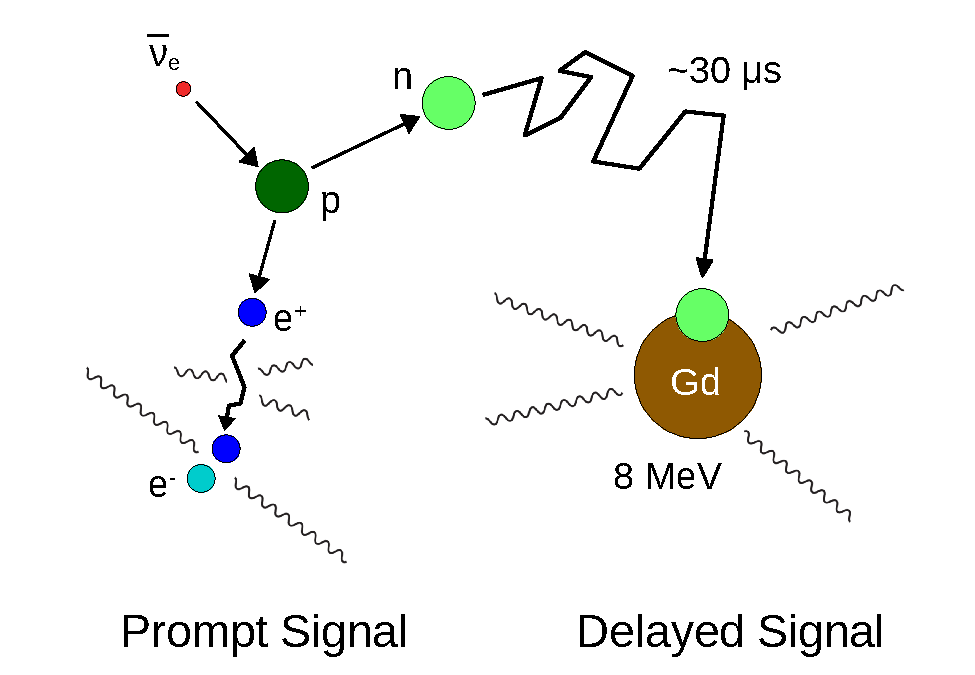
\includegraphics[width=0.65\textwidth]{Experiment/ibd_diagram.pdf}
  \caption{An illustration of the inverse beta decay reaction. Unlike a water Cherenkov detector, a Daya Bay AD cannot discern the direction of the positron.}
  \label{fig:expIBD}
\end{figure}

The kinematics of the IBD reaction are fairly straightforward. Essentially all of the antineutrino's energy $E_{\nubar}$ comes from its kinetic energy. During the interaction, some of this energy, equal to the neutron-proton mass difference $m_n - m_p$ (1.3~MeV) goes toward the conversion of the target proton into a neutron. An additional small amount of energy, on the order of 10~keV \cite{An_2017}, provides the recoil kinetic energy $K_n$ of the neutron. The conversion of the antineutrino into a positron consumes additional energy equal to the positron mass $m_e$ (511~keV). All of the remaining energy takes the form of the positron's kinetic energy $K_{e^+}$. Thus,
\begin{equation}
  K_{e^+} = E_{\nubar} - (m_n - m_p) - m_e - K_n
\end{equation}
After depositing its kinetic energy via ionization of the scintillator, the positron annihilates with an electron, releasing a pair of gamma rays with a total energy of $2m_e$. These gamma rays then undergo Compton scattering and/or photoelectric absorption, and the scintillator is further ionized by the kinetic energy of the resulting electrons. The total deposited energy $E_{\mathrm{dep}}$ is then
\begin{align*}
  E_{\mathrm{dep}} &= K_{e^+} + 2m_e \\
             &= E_{\nubar} + m_e - (m_n - m_p) - K_n.
\end{align*}
Since the energy resolution of the AD is, in the worst case (i.e. around 1~MeV), about 10\% (or 100~keV) \cite{An_2017}, the O(10~keV) kinetic energy of the neutron can be safely neglected. Using the fact that
\begin{equation}
  (m_n - m_p) - m_e \approx \SI{0.8}{MeV},
\end{equation}
we finally find that
\begin{equation}
  \label{eq:enuToEdep}
  E_{\mathrm{dep}} \approx E_{\nubar} - \SI{0.8}{MeV}.
\end{equation}
The energy threshold for the IBD reaction is equal to the amount of energy needed to produce the positron and to convert the proton into a neutron:
\begin{align*}
  E_{\nubar,\mathrm{min}} &= (m_n - m_p) + m_e \\
                    &\approx 1.3 + \SI{0.5}{MeV} \\
                    &= \SI{1.8}{MeV}.
\end{align*}
Using \autoref{eq:enuToEdep}, it then follows that
\begin{equation}
  E_{\mathrm{dep},\mathrm{min}} = \SI{1.0}{MeV}.
\end{equation}
Of course, this is also apparent from the simple fact that a threshold positron, with zero kinetic energy, will deposit an energy equal to $2m_e$, or $\sim$1.0~MeV. Given the finite energy resolution of the detector, some of these events will be reconstructed below 1.0~MeV. As such, a standard prompt-energy cut of 0.7~MeV is used in the official Daya Bay oscillation analyses, corresponding to about 3$\sigma$ below the 1.0~MeV peak. In \autoref{chap:cutVary}, we explore the effects of modifying this 0.7~MeV cut.

\section{Water pools and muon system}
\label{sec:expShieldVeto}

\begin{figure}[ht]
  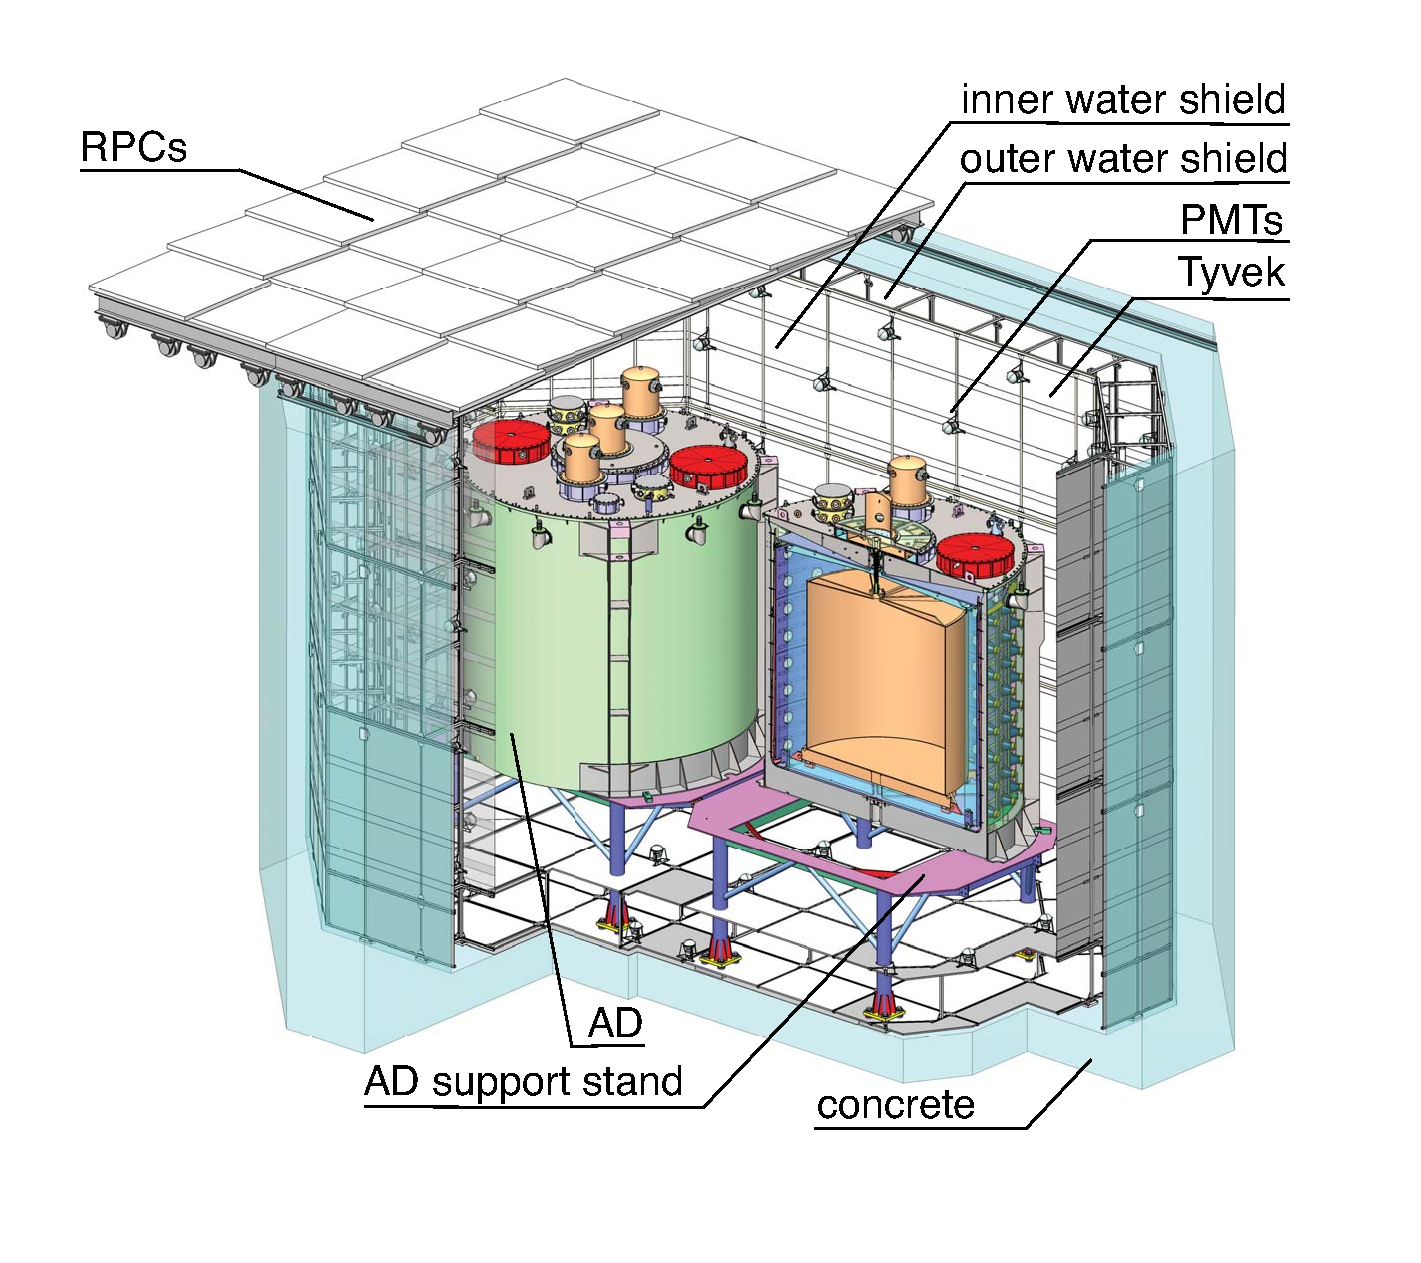
\includegraphics[scale=0.4]{exp_near_site_diagram.pdf}
  \caption{Water pool (including ADs) as configured in the near halls. The far hall is similar, with four ADs instead of two. From \cite{An_2017}.}
  \label{fig:expPool}
\end{figure}

Within each experimental hall, the ADs are immersed inside an instrumented pool of ultra-pure water. The water pools serve two purposes: First, to shield the ADs against both ambient $\gamma$ radioactivity and muon-induced neutrons from the surrounding rock, and second, to detect cosmic-ray muons that pass within the vicinity of the ADs. With respect to shielding, the $\sim$2.5~m-thick layer of water surrounding the ADs provides a $\sim10^6$ reduction in the rate of PMT hits from rock radioactivity \cite{Hack_2014}; without this suppression, antineutrino detection would be impossible.

Meanwhile, muon detection was accomplished by using PMTs\footnote{The water pool PMTs consisted of 619 Hamamatsu R5912 PMTs, as used in the ADs, as well as 341 EMI 9350KA and D642KB PMTs recycled from the MACRO experiment. The MACRO PMTs ultimately proved to be somewhat failure-prone, but not to the point of degrading the overall muon detection efficiency.} to observe the Cherenkov light produced when muons traverse the water. In order to allow for cross-checking of the muon system \cite{Hack_2014}, the water pools were divided by Tyvek sheets into two optically isolated zones, the \emph{inner} and \emph{outer water pools} (IWP/OWP). The IWP is instrumented by inward-facing PMTs protruding from the Tyvek, while the OWP is instrumented by both outward-facing PMTs on the Tyvek and inward-facing PMTs on the walls. The EH1 and EH2 water pools are essentially identical, while the EH3 pool was twice as wide in order to accommodate four detectors (in a $2\times2$ arrangement) instead of two. The number of PMTs in each water pool is listed in \autoref{tab:waterPoolPMTs} The FEE and trigger systems for the water pools are the same as those for the ADs, but the trigger configuration is different: ESUM is not used, and the NHIT thresholds are $\geq$6 for the IWP and $\ge$7 (8) for the near (far) hall OWP. Offline, in software, more stringent cuts (e.g., NHIT $\geq$ 12) were used as the definition of a muon event (see \autoref{tab:wpTriggerRates} for typical trigger rates in the muon system); AD events were then ignored in the immediate aftermath of such muons, greatly reducing muon-induced IBD-like backgrounds (especially neutrons).

\begin{table}[h]
  \begin{tabular}{lcc}
    \toprule
    Hall & IWS PMTs & OWS PMTs \\
    \midrule
    EH1 & 121 & 167 \\
    EH2 & 121 & 167 \\
    EH3 & 160 & 224 \\
    \bottomrule
  \end{tabular}
  \caption{The number of PMTs in each water pool \cite{AN2016133}.}
  \label{tab:waterPoolPMTs}
\end{table}

\begin{table}[h]
  \begin{tabular}{lc}
    \toprule
    Detector & Trigger rate (Hz) \\
    \midrule
    EH1-IWP & 220 \\
    EH1-OWP & 325 \\
    EH1-RPC & 215 \\
    \midrule
    EH2-IWP & 192 \\
    EH2-OWP & 245 \\
    EH2-RPC & 103 \\
    \midrule
    EH3-IWP & 39 \\
    EH3-OWP & 54 \\
    EH3-RPC & 36 \\
    \bottomrule
  \end{tabular}
  \caption{Typical trigger rates for the muon system, as given in \cite{AN2016133}.}
  \label{tab:wpTriggerRates}
\end{table}

Additional muon detection was provided by an assembly of modular resistive plate chambers (RPCs) mounted on a rolling frame on top of each water pool. Each module, approximately 2.2~m square and 8~cm thick, contained four layers of Bakelite sheets instrumented by eight readout strips, oriented alternatingly (between layers) in the x and y directions. The RPCs thus provide the 2D coordinate, at around 10~cm resolution, of each muon track that intersects the RPC plane. Two additional \emph{telescope} modules were installed in each hall along the center of opposing long edges of the water pool, to allow for high-angular-resolution tracking of a subset of muons in muon-related studies. The RPCs used HV, FEE, and trigger electronics distinct from those used by the AD and WP PMTs, with a trigger being issued whenever three out of four layers in a module are above threshold. Although the RPCs proved to be extremely useful in studies of muons and muon-induced backgrounds, they are not used in the analysis described in this thesis, as the water pools alone were sufficient to detect muons with effectively 100\% efficiency.

\section{Operations}
\label{sec:expOperations}

The operational procedures at Daya Bay are intended to ensure that data is recorded continuously, with minimal interruptions. As such, the majority of time is spent with the DAQ recording so-called \emph{Physics} runs, with the standard NHIT, ESUM, and prescaled trigger settings discussed in \autoref{sec:expPmtElec}. Each hall has a separate DAQ, so in general, three Physics runs were being taken in parallel at any given time. A typical Physics run lasts from 1--7 days, with a trend toward longer runs later in the experiment. Physics runs are generally ended either to perform maintenance or repairs, or to conduct calibration runs (discused shortly). Due to the large volume of data collected in each run, the DAQ does not emit a single data file for the run, but instead outputs a new file after roughly 1~GB of data has been accumulated, corresponding to 10--15 (30--40) minutes in the near (far) halls. Individual data files are thus identified by the \emph{run number} (taken from an incrementing counter common among all halls) and the \emph{file number} (which, for each run, ranges from 1 up to the total number of files in the run).

Every time the onsite DAQ emits a data file, it is stored temporarily on disk, where it is detected by a custom data transfer service known as SPADE. At this point, SPADE then initiates a transfer of the file to an offsite permanent storage facility at IHEP in China, where the file is categorized and stored. A second instance of SPADE, running at IHEP, then transfers the file to permanent storage at NERSC in the US. As a result, two redundant long-term copies of each data file are stored shortly after the data has been recorded.

Each Friday morning, ongoing Physics runs are stopped in order to perform a weekly set of calibration, or \emph{ADCalib} runs. These runs make use of the three automated calibration units (ACUs) located at the top of each AD. ACU A is located above the center, ACU B lies near the edge of the GdLS, and ACU C is situated above the LS. Each ACU features a turntable containing multiple calibration sources. The turntable rotates in order to select a particular source, which is then lowered by a cable, at an operator-specified height, into the liquid volume.

The sources deployed by each ACU include an LED (contained within a diffuser ball), a $^{60}$Co source (producing 1.17 and 1.33~MeV gamma rays), a $^{68}$Ge source (producing positrons), and a $^{241}$AmC-$^{13}$C source (producing low-rate neutrons). The $^{241}$AmC-$^{13}$C sources were always co-deployed with the $^{60}$Co and $^{68}$Ge sources, and were removed from ACUs B and C of every AD during commissioning of EH2-AD2 and EH3-AD4, so as to reduce correlated backgrounds from the AmC sources (\autoref{sec:bkgAmC}).

A typical Friday calibration campaign, lasting for about three hours, consisted of LED, $^{60}$Co (plus $^{241}$AmC-$^{13}$C), and $^{68}$Ge (plus $^{241}$AmC-$^{13}$C) runs, using all three ACUs at $\sim$8 vertical positions ranging from the top to the bottom of the AD. Of these runs, only the $^{60}$Co runs were used in regular calibration procedures, namely, the energy scale calibration of the so-called \emph{AdScaled} reconstruction algorithm, which we do not employ in this analysis. The other types of calibrations were useful for various studies of detector response (and, in the case of LED runs, for recalibrating the timing characterstics of each channel following a change in the electronics, as discussed in \autoref{sec:calibTiming}). In this analysis, the calibration runs are not used directly; as detailed in \autoref{chap:calib}, channel gains are calibrated using \emph{in situ} dark noise, and the energy scale of our chosen reconstruction (\emph{AdSimple}) uses spallation neutrons recorded during ordinary Physics runs.

Additional non-Physics runs, taken briefly and occasionally, included \emph{Pedestal} runs, used for monitoring the baselines of the ADCs, \emph{FEEDiag} runs, used for collecting diagnostic data from the electronics, and \emph{MOMonitor} runs, for monitoring the clarity of the mineral oil. None of these run types are relevant for this analysis.

In contrast to the ``fast'' operations of the DAQ, an auxiliary \emph{slow control} system (the Detector Control System, or DCS) was used for monitoring and controlling the environment in which the experiment operated. Most notably, the DCS was responsible for the high voltage (HV), allowing the HV to be enabled, disabled, and fine-tuned in order to achieve the desired gains. The DCS also incorporated a number of sensors to record temperature, humidity, barometric pressure, radon concentrations, water pressure, liquid levels in the overflow tanks, and various parameters of the gases above the liquids; cameras were also connected in order to visually monitor the interiors of the detectors. Any time the sensors would detect a deviation outside of the expected range, an alarm would be raised. These alarms would be noted by the weekly \emph{shifter} (the individual drafted with monitoring the experiment) and, if necessary, the appropriate expert would be consulted in order to correct any issues. In this way, the experiment was kept operating under the conditions needed to ensure quality of data. Control of temperature was particularly important, since any variations in the density of the GdLS target would affect the absolute antineutrino detection efficiency. Fortunately, the DCS enabled the temperature to be maintained within an adequately tight range, eliminating this source of potential bias.

\subfilebackmatter

\end{document}